\chapter{Wielowymiarowe zmienne losowe}
W klasycznym studium doboru struktury portfela (\cite{Markovitz_MPT}), Markovitz analizuje portfel aktywów. Przedmiotem tej pracy jest opis sposobu, w jaki indywidualne pozycje w portfelu wpływają na jego całościowy zwrot i ryzyko. Współczesna teoria portfela która została zapoczątkowana tą pracą wymaga zamodelowania całego systemu jakim jest zbiór akcji w portfelu. Markovitz pokazuje w swojej pracy istotę współzależności między poszczególnymi aktywami, od której zależy czy ryzyko portfela ulega dywersyfikacji, czy jest amplifikowane. Modelowanie każdego aktywa z osobna jest niewystarczające, ponieważ istota ich wpływu na portfel tkwi w przeważającym stopniu we współzależnościach pomiędzy nimi.\\
Problem wielowymiarowości i poprawnego jej opisu pojawia się nie tylko w finansach, ale w prawie każdej dziedzinie gdzie do realnych problemów aplikuje się modelowanie matematyczne. Zanim wprowadzimy więc pojęcie kopuły, które posłuży nam do analizy wielowymiarowych zależności, w tym rozdziale skupimy się na $d$-wymiarowych wektorach losowych $\mathbf{X} = [X_1, X_2, \dots, X_d]$ i przypomnimy elementy rachunku prawdopodobieństwa i statystyki istotnych z punktu widzenia teorii kopuł.\\

\section{Zmienne losowe}
\label{sec:rozklady_laczne}
Rozpatrywać będziemy przestrzeń probabilistyczną $(\Omega,\mathcal{F},\Pra)$, czyli niech $\Omega$ to pewien niepusty zbiór, $\mathcal{F}$ to $\sigma$-ciało zdarzeń losowych, a $\Pra$ to funkcja $\Pra\colon\Omega\rightarrow[0,1]$. 

\begin{df}[\textit{n}-wymiarowa zmienna losowa]
	\label{df:n_wym_zmienna_losowa}
	\textit{n}-wymiarową zmienną losową nazywamy funkcję określoną na przestrzeni zdarzeń elementarnych $\Omega$ i przyjmującą wartości rzeczywiste:
	
	$$ X\colon \Omega \mapsto \mathbb{R}^{n}, $$

	taką, że
	
	$$ \{ \omega \colon X(\omega) < x) \} \in \mathcal{F},$$
	
	dla każdego $x \in \R.$
\end{df}

W całej pracy zakładać będziemy że poruszamy się w przestrzeni zmiennych ciągłych, ponieważ dotykać będziemy problematyki danych rynkowych o takim charakterze. Teoria kopuł jest rozwinięta co prawda również dla zmiennych dyskretnych (\cite{Genest_Discrete_Copulas}) i dorobiła się już ciekawych aplikacyjnych prac (np. \cite{Koopman_DiscreteCopula_HTF}, czy \cite{Shefzik_Weather}), jednak literatura jest tu zdecydowanie uboższa. Do opisu interesujących nas rozkładów dostępne będziemy więc mieć analityczne postaci ich dystrybuanty lub gęstości. Ponieważ często podaje się różne ich parametryzacje, w tabeli \ref{tab:przykladowe_zmienne_losowe} podajemy gęstości zmiennych losowych przewijających się w tej pracy. Ich wykresy widoczne są na wykresie \ref{fig:przykladowe_zmienne_losowe}.

Warto wspomnieć, że istnieją również użyteczne rozkłady, które nie dają się wyrazić za pomocą gęstości czy dystrybuanty. Najpopularniejszym przykładem mogą być rozkłady stabilne, gdzie jedyne czym może my się posługiwać to funkcja charakterystyczna.  \cite{Stable_Distributions1}, czy \cite{Stable_Distributions2} podają bardzo dobry przegląd teorii rozkładów stabilnych i pokazują ich przewagę w kontekście modelowania nie-gaussowskich zwrotów na rynkach finansowych.

\begin{table}[h]
	\caption{\textbf{Popularne jednowymiarowe zmienne losowe.} Tabela przedstawia dystrybuanty, oraz gęstości popularnych jednowymiarowych zmiennych losowych pojawiających się w tej pracy.}
	\label{tab:przykladowe_zmienne_losowe}
	\centering
	\begin{tabular}{ll|c|c}
		\hline
		\textbf{Rozkład} & \textbf{Oznaczenie} & \textbf{Nośnik} & \textbf{Gęstość} \\
		\hline
		Normalny & $\mathcal{N}(\mu, \sigma)$ & $\mathbb{R}$ & $\frac{1}{\sigma \sqrt{2 \pi}} \exp\big(-\frac{(x-\mu)^2}{2\sigma^2}\big)$\\ 
		T-studenta & $\text{t}(\mu, \sigma, \nu)$ & $\mathbb{R}$ & $ \frac{\Gamma(\frac{\nu + 1}{2})}{\Gamma(\frac{\nu}{2})\sqrt{\pi\nu}\sigma} \bigg[1 + \big(\frac{x - \mu}{\sigma}\big)^2\frac{1}{\nu}\bigg]^{-\frac{\nu + 1}{2}} $ \\ 
		Beta & $\text{Beta}(\alpha, \beta)$ & $[0, 1]$ & $ x^{\alpha - 1}(1 - x)^{\beta - 1}\frac{\Gamma(\alpha + \beta)}{\Gamma(\alpha)\Gamma(\beta)}$ \\ 
		Wykładniczy & $\text{Exp}(\lambda)$ & $\mathbb{R}^{+}$ & $ \lambda e^{-\lambda x}$ \\
		Gamma & $\mathcal{G}(\alpha, \beta)$ & $\mathbb{R}^+$ & $x^{\alpha - 1}e^{-\beta x}\frac{\beta^\alpha}{\Gamma(\alpha)}$\\ 
		
		\hline
	\end{tabular}
\end{table}

\begin{figure}[H]
	\centering
	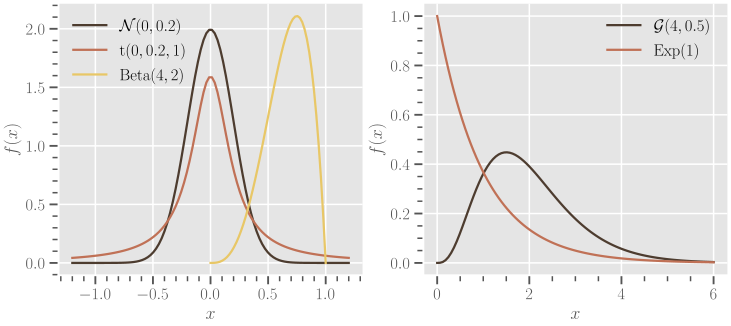
\includegraphics[width=\linewidth]{01_Rozklady_1D}
	\caption{\textbf{Jednowymiarowe zmienne losowe.} Przykładowe gęstości zmiennych losowych z tabeli \ref{tab:przykladowe_zmienne_losowe}.\label{fig:przykladowe_zmienne_losowe}}
\end{figure}

Do opisu zmiennych losowych \emph{wielo}wymiarowych, oprócz gęstości łącznej rozkładu wyróżniamy dodatkowo gęstości warunkowe i brzegowe. Opisują one jak zachowuje się współrzędna wektora losowego, jeśli pozostałe z nich przyjmą pewne wartości, lub jeśli kompletnie wyłączymy ich wpływ.

\begin{df}[Rozkłady brzegowy]
	Rozpatrzmy d-wymiarową zmienną losową $\mathbf{X} = [X_1, X_2, \dots, X_d]$ o gęstości $f(x_1, \dots, x_d)$. Gęstość rozkładu brzegowego $X_j$ definiujemy jako:
	$$f_j(x_j)=\int_{-\infty}^{\infty}\dots\int_{-\infty}^{\infty} f(x_1, \dots, x_{j-1}, x, x_{j+1}, \dots, x_d)  dx_1\dots dx_{j-1} dx_{j+1} \dots dx_d.$$
\end{df}

\begin{df}[Rozkład warunkowy]
	Rozpatrzmy d-wymiarową zmienną losową $\mathbf{X} = [X_1, X_2, \dots, X_d]$ o gęstości $f(x_1, \dots, x_d)$. Gęstość rozkładu warunkowego $X_j \vert X_k$ definiujemy jako:
	$$f_{j|k}(x_j|x_k) = \frac{f(x_1, \dots, x_d)}{f_k(x_k)}.$$
\end{df}


\section{Rozkłady wielowymiarowe}
\label{sec:rozklady_wielowymiarowe}
Naturalnym jest więc, że w praktyce często rozważamy modele wielowymiarowych zmiennych losowych, które mają regularne, łatwe do opisania gęstości łączne. Rozkłady jednowymiarowe z tabeli \ref{tab:przykladowe_zmienne_losowe} w naturalny sposób znajdują swoje rozszerzenia na więcej wymiarów (\cite{MultivariateDistributions}, \cite{Cherubini_Copula_Methods_in_Finance}). Najpopularniejszym tego przykładem jest rodzina $d$-wymiarowych rozkładów eliptycznych, do której należą rozkłady o gęstości postaci:

$$ f_{\mathcal{N}}(x, \mu, \Sigma) = k_d \vert\Sigma\vert^{-0.5}g\big((x-\mu)^T\Sigma^{-1}(x-\mu)\big).$$

W powyższej reprezentacji, $k_d \in\mathbb{R}$ jest stałą zależną od wymiaru, $\mu$ jest $d$-wymiarowym wektorem średnich, $\Sigma \in \mathbb{R}^{d \times d}$ to symetryczna, dodatnio zdefiniowana macierz, a $g \colon [0, \infty) \mapsto [0, \infty)$ jest pewną funkcją która nie zależy od wymiaru wektora.

Dla odpowiednio dobranych $g$ i $k_d$ otrzymamy w tej rodzinie wielowymiarowy rozkład normalny, czy wielowymiarowy rozkład t. Powstają one przy odpowiednio $k_d=(2\pi)^{-0.5d}$ i $g(s) = \exp(-0.5 t)$, lub $k_d=\Gamma(\frac{\nu + d}{2})/\Gamma(\frac{\nu}{2})$ i $g(s) = \big(1 + \frac{t}{\nu})^{-(\nu + d)/2}$.
\begin{figure}[H]
	\centering
	\includegraphics[width=0.45\linewidth]{01_MultivariateGaussian}	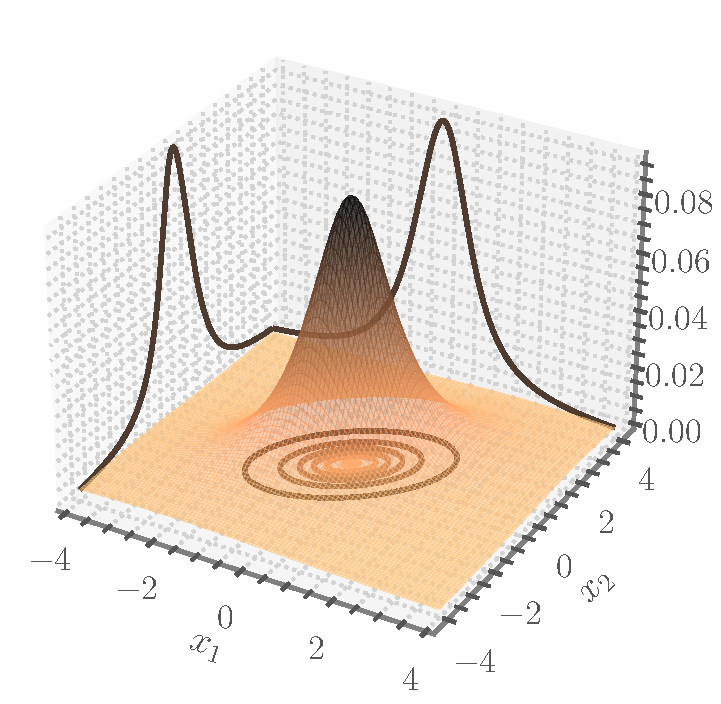
\includegraphics[width=0.45\linewidth]{01_MultivariateStudent}
	\caption{\textbf{Rozkłady eliptyczne.} Gęstości przykładowych rozkładów eliptycznych ($d=2, \mu=[0, 0], \Sigma = \big[\begin{smallmatrix}2&1\\1&2\end{smallmatrix}\big]$). Lewy panel: $2$-wymiarowy rozkład normalny. Prawy panel: $2$-wymiarowy rozkład t ($\nu = 0.5$).\label{fig:multivariate_gaussian_student}}
\end{figure}

Używając rozkładów eliptycznych implikujemy model w którym rozkłady brzegowe pochodzą z tej samej rodziny. Obserwując rysunek \ref{fig:multivariate_gaussian_student}, można rozpoznać charakterystyczne kształty rozkładów brzegowych. Manipulując różnymi rozkładami eliptycznymi możemy więc zamodelować różne struktury korelacji między zmiennymi, czy też ciężkość ogonów, lecz tracimy swobodę wyboru rozkładów brzegowych. \cite{Markovitz_MPT} i jego model bazują właśnie na rozkładzie multinormalnym ponieważ zakładają, że wektor średnich i macierz korelacji wystarczająco opisuje rozkład zwrotów aktywów rynkowych. Podejście to łatwo obalić ze względu na empiryczne dowody ciężkoogonowego charakteru zachowania rynku akcji (\cite{Taleb_BS_is_BS}, \cite{Mandelbrot_NonGaussianity}), czy zjawiska niesymetrycznej, silniejszej korelacji w lewym ogonie (\cite{Taleb_BS_is_BS}, \cite{AssymetricEquityDependency}). Nie mniej jednak nie da się odmówić, że ten prosty model jest wystarczający aby uświadomić jak istotny jest wpływ zależności komponentów na zachowanie całego systemu.\\


\section{Miary współzależności}
\label{sec:miary_współzależności}
Problemem w poprawnym opisie zależności między zmiennymi losowymi jest fakt, że dostępnych mamy wiele statystyk które ją mierzą. Każda z nich uchwyca pewien konkretny aspekt współzależności, i nie da się jasno wyróżnić konkretnej jako ,,najlepszej". W tej sekcji pracy zaprezentujemy wybrane narzędzia służące do badania struktury zależności zmiennych losowych.

\subsubsection{$\rho$ Pearsona}
Podstawową i najbardziej znaną miarą współzależności zmiennych losowych jest korelacja Pearsona.

\begin{df}[Korelacja Pearsona]
	Niech $X$ i $Y$ będą zmiennymi losowymi o skończonych drugich momentach. Współczynnikiem korelacji pearsona $\rho$ nazywamy
	
	$$ \rho(X, Y) \coloneqq \Corr(X,Y) = \frac{\Cov(X,Y)}{\sqrt{\Var(X)}\sqrt{\Var(Y)}}.$$
\end{df}

Ten współczynnik korelacji przyjmuje wartości z zakresu $[-1, 1]$, gdzie $\vert\rho\vert=1$ oznacza idealną liniową relację. Korelacja pearsona jest podstawową miarą zależności podawaną w każdym podręczniku do statystyki. Ma jednak szereg wad: nie jest zdefiniowana dla ciężkoogonowych rozkładów (przez nieokreśloną wariancję), oraz jest wrażliwa na monotonicznie rosnące przekształcenia $X$ i $Y$. Te i wiele innych ograniczeń korelacji pearsona stoi w sprzeczności z aksjomatycznym podejściem do miar zgodności (czyt. \ref{def:miara_zgodnosci}). \\
Gdy w rozdziale \ref{subsec:dwuwymiarowe_kopuly_definicja} zdefiniujemy czym jest główny obiekt tej pracy, czyli kopuła, zależeć nam będzie, żeby móc opisać zależność zmiennych losowych $X$, $Y$ w terminach łączącej je kopuły $C$. Z tego powodu, interesujące dla nas będą miary zależności, które są niezmiennicze na monotonicznie rosnące przekształcenia (ze względu na transformację PIT \ref{def:PIT}, czyt. rozdział \ref{subsec:dwuwymiarowe_kopuly_definicja}). Korelacja pearsona nam tego nie zapewni, ale możemy zdefiniować inne miary: zgodności zmiennych losowych, które posiadają lepsze własności z punktu widzenia teorii kopuł.\\

Aby w pełni zdefiniować aksjomatyczne podejście do miar zgodności jak wprowadził to Scarsini w \cite{Scarsini1984}, potrzebujemy mieć dostępne pojęcie kopuły. W tej pracy formalnie zostaną one wprowadzone dopiero w definicji \ref{def:bivariate_copula}, w związku z czym na ten moment powiemy jedynie (nieformalnie), że kopuła jest funkcją która opisuje charakter i siłę zależności między zmiennymi losowymi. Pełną definicję i opis czym są kopuły można przeczytać w rozdziale \ref{sec:dwuwymiarowe_kopuly}.

\begin{df}[Miara zgodności]
	Rozpatrzmy zmienne losowe $X$ i $Y$ powiązane kopułą $C$. $M_{X,Y}=M_C$ nazwiemy miarą zgodności, wtedy i tylko wtedy gdy:
	\begin{enumerate}
		\item jest zdefiniowana dla dowolnych zmiennych $X$, $Y$
		\item jest relatywna, lub znormalizowana: $M_{X,Y}\in[-1,1]$
		\item jest symetryczna: $M_{X,Y}=M_{Y,X}$
		\item jeśli $X$ i $Y$ są niezależne, to $M_{X,Y}=0$
		\item $M_{-X,Y}=M_{X,-Y}=-M_{Y,X}$
		\item jest zbieżna, gdy kopuła jest punktowo zbieżna, tzn. jeśli $\{(X_n,Y_n)\}$ jest ciągiem ciągłych zmiennych losowych o kopułach $\{C_n\}$, oraz 
		$$ \lim\limits_{n\to\infty} C_n(u, v) =C(u, v)\text{, dla każdych }(u, v)\in[0,1]^2,$$
		to wtedy
		$$ \lim\limits_{n\to\infty}M_{X_n,Y_n}=M_{X,Y}.$$
		\item przestrzega relacji zgodności: jeśli $C_1(u,v) \leqslant C_2(u,v)$ dla wszystkich $(u, v)\in[0,1]^2$, to $M_{C_1} \leqslant M_{C_2}.$
	\end{enumerate}
	\label{def:miara_zgodnosci}		
\end{df}

Aksjomatyczne podejście z powyższej definicji zawęża przestrzeń miar zgodności do takich, które są niezmiennicze względem rosnących transformacji, czyli:
$$ M_{X,Y} = M_{\alpha(X), \beta(Y)},$$
dla dowolnych funkcji $\alpha,\beta$ rosnących prawie wszędzie.\\

\subsubsection{Współmonotoniczność i przeciwmonotoniczność}
Współmonotoniczność i przeciwmonotoniczność to szczególne przypadki zależności zmiennych losowych, w których są one od siebie perfekcyjnie zależne.

\begin{df}[Zbiór współmonotoniczny]
	Zbiór $A \subset \R^2$ nazywamy współmonotonicznym, wtedy i tylko wtedy gdy dla dowolnych $(x_1, y_1)$, $(x_2, y_2)$ z $A$ zachodzi:
	
	$$ (x_1 - y_1)(x_2 - y_2) >0.$$
\end{df}

\begin{df}[Zbiór przeciwmonotoniczny]
	Zbiór $A \subset \R^2$ nazywamy przeciwmonotonicznym, wtedy i tylko wtedy gdy dla dowolnych $(x_1, y_1)$, $(x_2, y_2)$ z $A$ zachodzi:
	
	$$ (x_1 - y_1)(x_2 - y_2) <0.$$
\end{df}


\begin{df}[Zmienne losowe współ- i przeciwmonotoniczne]
	Wektor losowy $(X, Y)$ nazywamy współmonotonicznym (przeciwmonotonicznym), lub perfekcyjnie dodatnio (ujemnie) zależnym wtedy i tylko wtedy gdy istnieje zbiór współmonotoniczny (przeciwmonotoniczny) $A\subset\R^2$:
	
	$$ \Pra[(X,Y)\in A]=1.$$
\end{df}

Współmonotoniczność i przeciwmonotoniczność zmiennych losowych jest ważnym konceptem w teorii kopuł, ponieważ definiuje najsilniejszy rodzaj zależności jakie kopuły mogą reprezentować (czyt. twierdzenie \ref{thm:frechet_hoeffding}).

\subsubsection{$\tau$ Kendalla i $\rho$ Spearmana}

Współczynniki $\tau$ Kendalla i $\rho$ Spearmana oba spełniają aksjomaty miar zgodności z \cite{Scarsini1984}. Są współczynnikami rangowymi, więc nie zależą od monotonicznych przekształceń rozkładów brzegowych $X$ czy $Y$. Ich zaletą jest to, że mogą być przez to jednoznacznie przedstawione w języku kopuły - co znajduje zastosowanie przy estymacji parametrów modeli kopułowych. Ta własność zazwyczaj nie zachodzi w przypadku korelacji Pearsona.

\begin{df}[$\tau$ Kendalla]
	Współczynnik $\tau$ Kendalla między ciągłymi zmiennymi losowymi $X$ i $Y$ o kopule definiujemy jako:
	$$ \tau = \Pra[(X_1-X_2)(Y_1-Y_2)>0] - \Pra[(X_1-X_2)(Y_1-Y_2) <0], $$
	gdzie $(X_1, Y_1)$ i $(X_2, Y_2)$ są kopiami iid wektora $(X, Y)$.
\end{df}

\begin{df}[$\rho$ Spearmana]
	Współczynnik $\rho$ Spearmana między ciągłymi zmiennymi losowymi $X$ i $Y$ o rozkładach brzegowych $F_X$ i $F_y$ zadany jest przez:
	$$ \rho = \Corr[F_X(X), F_Y(Y)].$$
\end{df}

Współczynniki te dają się jednoznacznie wyrazić za pomocą kopuł łączących $X$~i~$Y$~-~własność tę podamy w rozdziale \ref{subsec:dwuwymiarowe_kopuly_definicja}. Istotny również jest fakt, że ich ekstremalne wartości, tj. $\rho= 1$, czy $\tau=1$ odpowiadają współmonotoniczności zmiennych losowych, a $\rho=-1$, czy $\tau=-1$ odpowiadają przeciwmonotoniczności.

\subsubsection{Zależność ogonów}
Na zależność zmiennych losowych można popatrzeć również ze strony zależności obserwacji ekstremalnych. Rozważmy następującą statystykę:

\begin{df}[Współczynnik zależności ogonów]
	Górnym współczynnikiem zależności ogonów $(X_1, X_2)$ o rozkładach brzegowych $F_1$ i $F_2$ i kopuli $C$ nazywamy:
	$$ \lambda^{u} = \lim\limits_{t\to1^{-}}\Pra[X_2 > F_2^{-1}(t) \vert X_1 > F_1^{-1}(t) ].$$
	Dolnym współczynnikiem nazywamy:
	$$ \lambda^{l} = \lim\limits_{t\to0^{+}}\Pra[X_2 \leqslant F_2^{-1}(t) \vert X_1 \leqslant F_1^{-1}(t) ].$$
\end{df}

Współczynniki zależności ogonów informują o sile zależności zmiennych losowych w granicy, gdy dążymy z jedną z nich coraz dalej w jej ogon. Mówimy, że zmienne losowe posiadają zależność ogonów jeśli $\lambda \in (0, 1]$, lub jej nie posiadają gdy $\lambda =0$. Te wspołczynniki zależą przede wszystkim od obserwacji będących ekstremalnymi względem obu zmiennych. Rysunek \ref{fig:tail_dependence} prezentuje przykładowy rozkład posiadający dolny współczynnik zależności ogonów, lecz nie posiadający górnego wspołczynnika. Kolorami zaznaczone są obserwacje które wpływają na dolny (szare punkty) i górny (czerwone punkty) współczynnik zależności ogonów.\\
W praktycznych zastosowaniach, jest on jednak trudny do kalibracji z danych - koncept ten działa raczej w drugą stronę: z parametrów skalibrowanego modelu implikowany jest współczynnik zależności ogonów.
\begin{figure}[H]
	\centering
	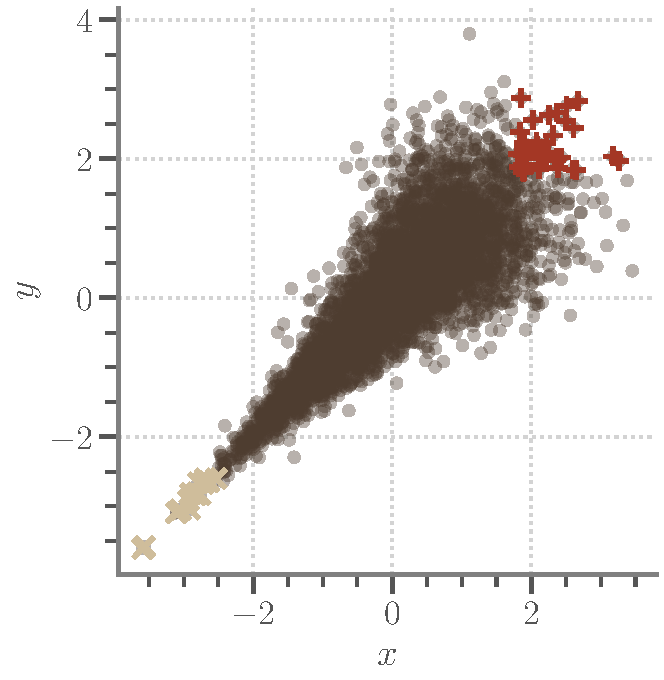
\includegraphics[width=0.5\linewidth]{01_Tail_dependence}	
	\caption{\textbf{Współczynnik zależności ogonów.} Rozkład o dolnym współczynniku i braku górnego współczynnika. Obserwacje zaznaczone na szaro wpływają na dolny współczynnik. Obserwacje zaznaczone na czerwono wpływają na górny współczynnik zależności ogonów.\label{fig:tail_dependence}}
\end{figure}

W tym rozdziale zdefiniowialiśmy różne miary pomagające nam zrozumieć zależność zmiennych losowych. Widzimy zatem, że korelacja Pearsona i modele eliptyczne to za mało, aby w pełni uchwycić charakter współzależności. W kolejnym rozdziale podamy teorię \emph{kopuł}, które dadzą nam odpowiednie narzędzia do walki z tym problemem.


\mgrclosechapter